\let\negmedspace\undefined
\let\negthickspace\undefined
\documentclass[journal]{IEEEtran}
\usepackage[a5paper, margin=10mm, onecolumn]{geometry}
%\usepackage{lmodern} % Ensure lmodern is loaded for pdflatex
\usepackage{tfrupee} % Include tfrupee package

\setlength{\headheight}{1cm} % Set the height of the header box
\setlength{\headsep}{0mm}     % Set the distance between the header box and the top of the text

\usepackage{gvv-book}
\usepackage{gvv}
\usepackage{cite}
\usepackage{amsmath,amssymb,amsfonts,amsthm}
\usepackage{algorithmic}
\usepackage{graphicx}
\usepackage{textcomp}
\usepackage{xcolor}
\usepackage{txfonts}
\usepackage{listings}
\usepackage{enumitem}
\usepackage{mathtools}
\usepackage{gensymb}
\usepackage{comment}
\usepackage[breaklinks=true]{hyperref}
\usepackage{tkz-euclide} 
\usepackage{listings}
% \usepackage{gvv}                                        
\def\inputGnumericTable{}                                 
\usepackage[latin1]{inputenc}                                
\usepackage{color}                                            
\usepackage{array}                                            
\usepackage{longtable}                                       
\usepackage{calc}                                             
\usepackage{multirow}                                         
\usepackage{hhline}                                           
\usepackage{ifthen}                                           
\usepackage{lscape}
\begin{document}

\bibliographystyle{IEEEtran}
\vspace{3cm}

\title{1.8.20}
\author{EE25BTECH11003 - Adharvan Kshathriya Bommagani}
% \maketitle
% \newpage
% \bigskip
{\let\newpage\relax\maketitle}

\renewcommand{\thefigure}{\theenumi}
\renewcommand{\thetable}{\theenumi}
\setlength{\intextsep}{10pt} % Space between text and floats
\textbf{Question}:\\
 Find a relation between x and y such that the point (x, y) is equidistant from the
point (3, 6) and (-3, 4).  
\bigskip

\textbf{Solution}:\\

\begin{align}
\text{Let } 
\vec{A} = \myvec{ 3 \\ 6 } \ \ ,\ \vec{B} = \myvec{ -3 \\ 4 }
\end{align}
 
The midpoint of the line segment $\vec{B}-\vec{A}$ is 

\begin{align}
    \vec{M} =& \frac{\vec{A}+\vec{B}}{2}\\
    \vec{M} =& \myvec{0 \\[1ex] 5}
\end{align}

Let a point on the perpendicular bisector of the line segment joining $\vec{A}$ and $\vec{B}$ be $\vec{P}$. 

\begin{align}
    \vec{P} = \myvec{x\\y}
\end{align}

\begin{align}
    \vec{P} - \vec{M} = \myvec{x\\[1ex] y-5}
\end{align}

$\vec{P}-\vec{M}$ is the perpendicular bisector of line segment $\vec{B}-\vec{A}$.

\begin{align}
    \brak{\vec{P}-\vec{M}}^\top\brak{\vec{B}-\vec{A}} = 0
\end{align}

\begin{align}
    \myvec{x&&y-5}\myvec{-6\\-2} = 0
\end{align}

\begin{align}
    -6x-2y+10=0\\
    y+3x=0
\end{align}

$\therefore$ The relation for the values of x and y such that (x,y) is equidistant from the point (3,6) and (-3,4).

\textbf{Graph of the line segment AB with midpoint M}
\begin{figure}[H]
    \centering
    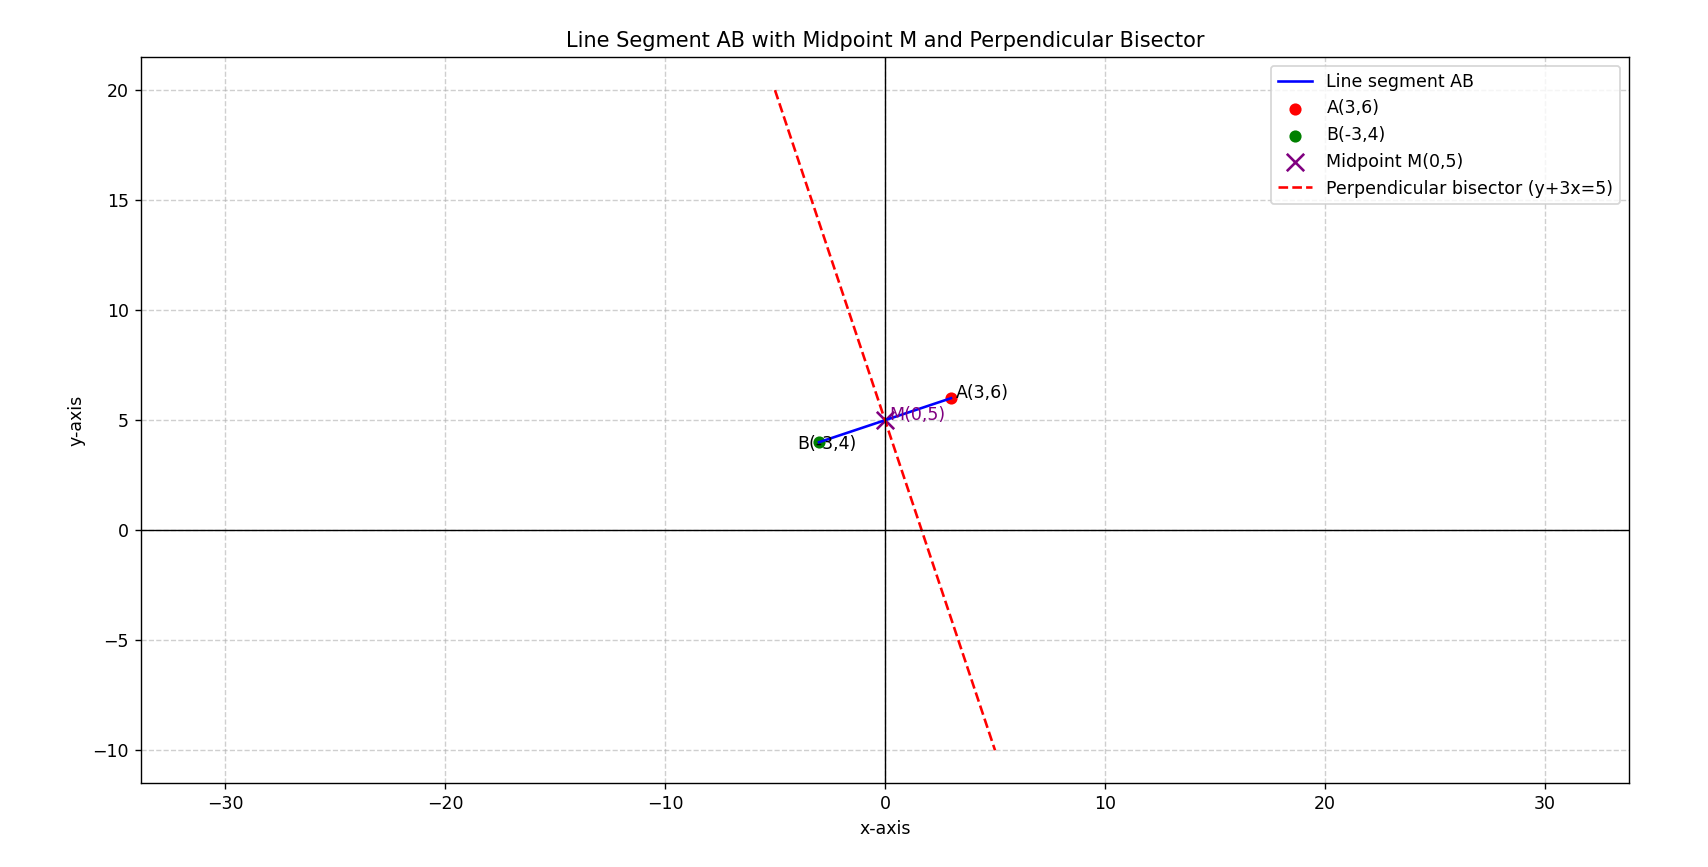
\includegraphics[width=1.1\columnwidth]{figs/fig1.png}
    \caption{Figure for 1.8.20}
    \label{fig1}
\end{figure}




\end{document}
























